\documentclass[tikz,margin=.1in]{standalone}
\usepackage{pgfplots,lmodern}
\pgfplotsset{compat=newest}

\begin{document}
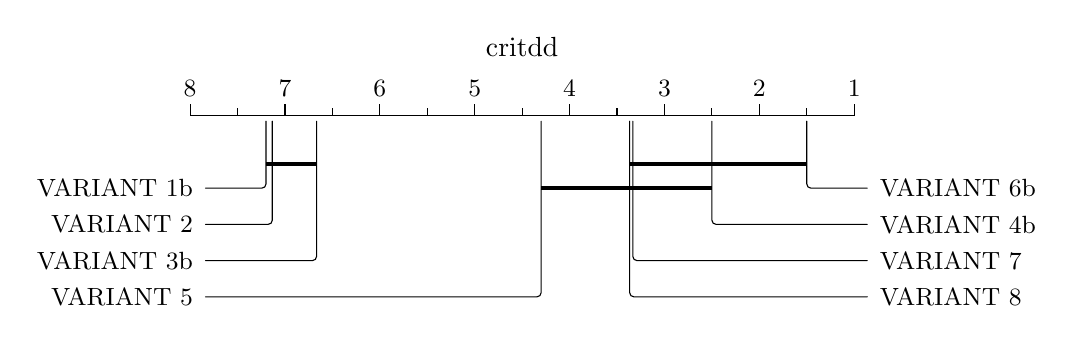
\begin{tikzpicture}[
  treatment line/.style={rounded corners=1.5pt, line cap=round, shorten >=1pt},
  treatment label/.style={font=\small},
  group line/.style={ultra thick},
]

\begin{axis}[
  clip={false},
  axis x line={center},
  axis y line={none},
  axis line style={-},
  xmin={1},
  ymax={0},
  scale only axis={true},
  width={\axisdefaultwidth},
  ticklabel style={anchor=south, yshift=1.3*\pgfkeysvalueof{/pgfplots/major tick length}, font=\small},
  every tick/.style={draw=black},
  major tick style={yshift=.5*\pgfkeysvalueof{/pgfplots/major tick length}},
  minor tick style={yshift=.5*\pgfkeysvalueof{/pgfplots/minor tick length}},
  title style={yshift=\baselineskip},
  xmax={8},
  ymin={-5.5},
  height={6\baselineskip},
  xtick={1,2,3,4,5,6,7,8},
  minor x tick num={1},
  x dir={reverse},
  title={critdd},
]

\draw[treatment line] ([yshift=-2pt] axis cs:1.5, 0) |- (axis cs:0.8333333333333334, -2.0)
  node[treatment label, anchor=west] {VARIANT 6b};
\draw[treatment line] ([yshift=-2pt] axis cs:2.5, 0) |- (axis cs:0.8333333333333334, -3.0)
  node[treatment label, anchor=west] {VARIANT 4b};
\draw[treatment line] ([yshift=-2pt] axis cs:3.3333333333333335, 0) |- (axis cs:0.8333333333333334, -4.0)
  node[treatment label, anchor=west] {VARIANT 7};
\draw[treatment line] ([yshift=-2pt] axis cs:3.3666666666666667, 0) |- (axis cs:0.8333333333333334, -5.0)
  node[treatment label, anchor=west] {VARIANT 8};
\draw[treatment line] ([yshift=-2pt] axis cs:4.3, 0) |- (axis cs:7.866666666666667, -5.0)
  node[treatment label, anchor=east] {VARIANT 5};
\draw[treatment line] ([yshift=-2pt] axis cs:6.666666666666667, 0) |- (axis cs:7.866666666666667, -4.0)
  node[treatment label, anchor=east] {VARIANT 3b};
\draw[treatment line] ([yshift=-2pt] axis cs:7.133333333333334, 0) |- (axis cs:7.866666666666667, -3.0)
  node[treatment label, anchor=east] {VARIANT 2};
\draw[treatment line] ([yshift=-2pt] axis cs:7.2, 0) |- (axis cs:7.866666666666667, -2.0)
  node[treatment label, anchor=east] {VARIANT 1b};
\draw[group line] (axis cs:6.666666666666667, -1.3333333333333333) -- (axis cs:7.2, -1.3333333333333333);
\draw[group line] (axis cs:2.5, -2.0) -- (axis cs:4.3, -2.0);
\draw[group line] (axis cs:1.5, -1.3333333333333333) -- (axis cs:3.3666666666666667, -1.3333333333333333);

\end{axis}
\end{tikzpicture}
\end{document}
